\documentclass[aspectratio=169,12pt,t]{beamer}

% --- Theme: Metropolis (modern, clean) ---
\usetheme[progressbar=frametitle,numbering=fraction,block=fill]{metropolis}

% --- Fira Sans font (install texlive-fonts-extra if missing) ---
\IfFileExists{FiraSans.sty}{\usepackage[sfdefault]{FiraSans}}{}

% --- Light background with warm accent ---
\definecolor{mDarkTeal}{RGB}{35,55,59}
\definecolor{mLightBrown}{RGB}{235,228,216}
\definecolor{mAccent}{RGB}{140,70,20}

\setbeamercolor{normal text}{fg=mDarkTeal,bg=white}
\setbeamercolor{alerted text}{fg=mAccent}
\setbeamercolor{frametitle}{bg=mDarkTeal,fg=white}
\setbeamercolor{progress bar}{fg=mAccent,bg=mLightBrown}
\setbeamercolor{title separator}{fg=mAccent}
\setbeamercolor{progress bar in head/foot}{fg=mAccent,bg=mLightBrown}
\setbeamercolor{progress bar in section page}{fg=mAccent,bg=mLightBrown}

% --- Packages ---
\usepackage[utf8]{inputenc}
\usepackage{amsmath,amssymb,amsthm}
\usepackage{mathrsfs}
\usepackage{tikz}
\usetikzlibrary{arrows.meta,positioning,calc,decorations.pathreplacing,shapes,patterns}
\usepackage{pgfplots}
\pgfplotsset{compat=1.18}

% --- Custom colors for content types ---
\definecolor{defcolor}{RGB}{25,85,120}
\definecolor{thmcolor}{RGB}{140,35,35}
\definecolor{proofcolor}{RGB}{35,100,50}
\definecolor{excolor}{RGB}{140,75,10}
\definecolor{remcolor}{RGB}{90,90,90}

% --- Beamer blocks for mathematical content types ---
\newenvironment{defblock}[1]{%
  \setbeamercolor{block title}{bg=defcolor,fg=white}%
  \setbeamercolor{block body}{bg=defcolor!5}%
  \begin{block}{#1}}{\end{block}}

\newenvironment{thmblock}[1]{%
  \setbeamercolor{block title}{bg=thmcolor,fg=white}%
  \setbeamercolor{block body}{bg=thmcolor!5}%
  \begin{block}{#1}}{\end{block}}

\newenvironment{proofblock}[1]{%
  \setbeamercolor{block title}{bg=proofcolor,fg=white}%
  \setbeamercolor{block body}{bg=proofcolor!5}%
  \begin{block}{#1}}{\end{block}}

\newenvironment{exblock}[1]{%
  \setbeamercolor{block title}{bg=excolor,fg=white}%
  \setbeamercolor{block body}{bg=excolor!5}%
  \begin{block}{#1}}{\end{block}}

\newenvironment{remblock}[1]{%
  \setbeamercolor{block title}{bg=remcolor,fg=white}%
  \setbeamercolor{block body}{bg=remcolor!5}%
  \begin{block}{#1}}{\end{block}}

% --- Metadata ---
\title{Chapter 1: The Real and Complex Number Systems}
\subtitle{Section: The Complex Field}
\author{Based on Walter Rudin's \emph{Principles of Mathematical Analysis}}
\date{}

\begin{document}

% =============================================================================
% TITLE AND OUTLINE
% =============================================================================

\begin{frame}
  \titlepage
  \note{
    Welcome to Chapter 1, Section 6: The Complex Field. In this section
    we construct the complex numbers from scratch, using nothing more than
    ordered pairs of real numbers. We will see that these ordered pairs,
    equipped with the right addition and multiplication rules, form a field.
    Along the way we will meet the imaginary unit i, the conjugate, the
    absolute value, and the important Schwarz inequality.
  }
\end{frame}

\begin{frame}{Outline}
  \tableofcontents
  \note{
    Here is our outline for this section. We begin with the definition of
    complex numbers and verify that they form a field. Then we show how
    the familiar notation a plus b i arises naturally. Next we study
    conjugation and the absolute value, establishing the triangle inequality.
    Finally, we prove the Schwarz inequality, which will be important
    throughout the rest of the book. Let's start with some motivation.
  }
\end{frame}

% =============================================================================
% MOTIVATION
% =============================================================================

\section{Definition and Field Structure}

% --- Build 1/3 ---
\begin{frame}{Why the Complex Numbers?}
  \begin{itemize}
    \item We have built $\mathbb{R}$ with the least upper bound property
  \end{itemize}

  \note{
    Let's begin with some motivation. In the previous sections we carefully
    constructed the real number system and established its key property: the
    least upper bound property. So the reals are a complete ordered field.
    Why would we want anything more? Well, there is a limitation.
  }
\end{frame}

% --- Build 2/3 ---
\begin{frame}{Why the Complex Numbers?}
  \begin{itemize}
    \item We have built $\mathbb{R}$ with the least upper bound property
    \item But not every polynomial has a root in $\mathbb{R}$ --- e.g., $x^2 + 1 = 0$
  \end{itemize}

  \note{
    The problem is that certain very simple equations have no solution in the
    reals. For instance, the equation x squared plus one equals zero has no
    real solution, since the square of any real number is nonnegative. This
    is a serious limitation if we want a number system where every polynomial
    equation can be solved. So how do we fix this?
  }
\end{frame}

% --- Build 3/3 ---
\begin{frame}{Why the Complex Numbers?}
  \begin{itemize}
    \item We have built $\mathbb{R}$ with the least upper bound property
    \item But not every polynomial has a root in $\mathbb{R}$ --- e.g., $x^2 + 1 = 0$
    \item Solution: extend $\mathbb{R}$ to the \alert{complex numbers} $\mathbb{C}$
  \end{itemize}

  \note{
    The solution is to extend the real numbers to a larger number system,
    the complex numbers. Rudin's approach is elegant: he defines complex
    numbers purely as ordered pairs of reals with specific arithmetic rules.
    No mysterious square root of negative one is assumed to exist. Let's see
    how this works.
  }
\end{frame}

% =============================================================================
% DEFINITION 1.24
% =============================================================================

\begin{frame}{Definition 1.24: Complex Number}
  \begin{defblock}{Definition 1.24}
    A \alert{complex number} is an ordered pair $(a, b)$ of real numbers.
  \end{defblock}

  \vspace{0.5em}
  \textbf{Equality:} $(a, b) = (c, d)$ if and only if $a = c$ and $b = d$.

  \note{
    Here is the formal definition. A complex number is simply an ordered
    pair of real numbers. The word ``ordered'' means that the pair "a", "b" and
    the pair "b", "a" are different whenever "a" is not equal to "b". Two complex
    numbers are equal precisely when both their first components and second
    components match. This may seem obvious, but Rudin points out that the
    definition is not entirely superfluous --- think of how equality of
    rational numbers works when they are represented as quotients of integers.
    Now let's define the arithmetic operations.
  }
\end{frame}

% --- Build 1/2 ---
\begin{frame}{Definition 1.24: Arithmetic Operations}
  Let $x = (a, b)$ and $y = (c, d)$.

  \vspace{0.5em}
  \textbf{Addition:}
  \[
    x + y = (a + c,\; b + d)
  \]

  \note{
    Now we define the arithmetic. Let "x" equal the pair "a", "b" and "y" equal the
    pair "c", "d". Addition is done component-wise: we add the first components
    and the second components separately. This is exactly what you would
    expect. Next, let's see the multiplication rule, which is more surprising.
  }
\end{frame}

% --- Build 2/2 ---
\begin{frame}{Definition 1.24: Arithmetic Operations}
  Let $x = (a, b)$ and $y = (c, d)$.

  \vspace{0.5em}
  \textbf{Addition:}
  \[
    x + y = (a + c,\; b + d)
  \]

  \textbf{Multiplication:}
  \[
    xy = (ac - bd,\; ad + bc)
  \]

  \note{
    Multiplication is more interesting. The first component of the product
    is "a" "c" minus "b" "d", and the second component is "a" "d" plus "b" "c". This formula
    may look strange at first, but it is exactly the rule you get if you
    formally multiply "a" plus "b" "i" times "c" plus "d" "i" and use the fact that
    "i" squared equals negative one. Of course, we haven't introduced "i" yet ---
    that comes later. For now, this is just a definition. Let's visualize
    these ordered pairs in the plane.
  }
\end{frame}

% --- Diagram: Complex plane ---
\begin{frame}{The Complex Plane}
  \begin{center}
  \begin{tikzpicture}[scale=1.4]
    % Axes
    \draw[->] (-0.3,0) -- (5,0) node[right]{Real axis};
    \draw[->] (0,-0.3) -- (0,3.5) node[above]{Imaginary axis};
    % Point z = (a, b)
    \fill[blue] (3,2) circle (2pt);
    \node[blue, above right] at (3,2) {$z = (a, b)$};
    % Dashed projections
    \draw[dashed, gray] (3,0) -- (3,2);
    \draw[dashed, gray] (0,2) -- (3,2);
    % Labels on axes
    \node[below] at (3,0) {$a$};
    \node[left] at (0,2) {$b$};
    % Origin
    \fill (0,0) circle (1.5pt);
    \node[below left] at (0,0) {$0$};
    % Arrow from origin to z
    \draw[-{Stealth}, thick, blue!70] (0,0) -- (3,2);
  \end{tikzpicture}
  \end{center}

  \note{
    We can visualize each complex number as a point in the plane. The
    horizontal axis represents the first component, which we will call the
    real part, and the vertical axis represents the second component, the
    imaginary part. The complex number "z" equals the pair "a", "b" corresponds to
    the point with coordinates "a" and "b". We can also think of "z" as a vector
    from the origin to that point. This geometric picture will be very
    helpful later when we discuss absolute values and the triangle inequality.
    Now let's verify that these arithmetic rules give us a field.
  }
\end{frame}

% =============================================================================
% THEOREM 1.25
% =============================================================================

\begin{frame}{Theorem 1.25: $\mathbb{C}$ Is a Field}
  \begin{thmblock}{Theorem 1.25}
    The set of all complex numbers, with the addition and multiplication
    of Definition 1.24, is a \alert{field}.

    \vspace{0.3em}
    The additive identity is $(0, 0)$ and the multiplicative identity is $(1, 0)$.
  \end{thmblock}

  \note{
    This is the main structural result. The complex numbers form a field.
    That means all the field axioms we listed back in Definition 1.12 are
    satisfied: commutativity and associativity of addition and multiplication,
    existence of identity elements and inverses, and the distributive law.
    The zero element is the pair zero, zero and the one element is the pair
    one, zero. The proof is a systematic verification of each axiom using the
    field properties of the reals. Let's look at the proof strategy.
  }
\end{frame}

\begin{frame}{Proof Strategy: Theorem 1.25}
  \textbf{Goal:} Verify all field axioms from Definition 1.12.

  \vspace{0.5em}
  \textbf{Approach:} Let $x = (a,b)$, $y = (c,d)$, $z = (e,f)$.

  \vspace{0.3em}
  \begin{tabular}{@{}ll}
    \textbf{(A1)--(A5)} & Addition: closure, commutativity, associativity, \\
                         & identity $(0,0)$, inverse $(-a,-b)$ \\[4pt]
    \textbf{(M1)--(M5)} & Multiplication: closure, commutativity, associativity, \\
                         & identity $(1,0)$, inverse $\tfrac{1}{x}$ \\[4pt]
    \textbf{(D)}         & Distributive law
  \end{tabular}

  \note{
    Here is the roadmap for the proof. We write "x" equals "a", "b", "y" equals
    "c", "d", and "z" equals "e", "f", and then verify each field axiom one by one.
    The addition axioms are straightforward since addition is component-wise.
    The multiplication axioms require more computation: associativity
    involves expanding lengthy products, and the existence of multiplicative
    inverses requires a clever formula. Let us walk through the key steps,
    starting with the addition axioms.
  }
\end{frame}

% --- Proof: Addition axioms ---
\begin{frame}{Proof of Theorem 1.25 --- Addition Axioms}
  \begin{proofblock}{Addition Axioms (A1)--(A5)}
    \textbf{(A2):} $x + y = (a+c,\, b+d) = (c+a,\, d+b) = y + x$

    \vspace{0.2em}
    \textbf{(A3):} $(x+y)+z = (a+c+e,\; b+d+f) = x+(y+z)$

    \vspace{0.2em}
    \textbf{(A4):} $x + (0,0) = (a,b) = x$

    \vspace{0.2em}
    \textbf{(A5):} Set $-x = (-a, -b)$. Then $x + (-x) = (0,0)$
  \end{proofblock}

  \note{
    The addition axioms follow directly from the corresponding properties of
    real number addition. Commutativity holds because real addition is
    commutative. Associativity works because we can regroup the real additions
    in each component freely. The pair zero, zero is the additive identity
    because adding zero to each component leaves the number unchanged. And
    the additive inverse of the pair "a", "b" is the pair negative "a", negative "b",
    since adding them gives zero, zero. Closure is clear since sums of real
    numbers are real. Now let's turn to the multiplication axioms, which are
    more interesting.
  }
\end{frame}

% --- Proof: Multiplication axioms ---
\begin{frame}{Proof of Theorem 1.25 --- Multiplication Axioms}
  \begin{proofblock}{(M2), (M3), (M4)}
    \textbf{(M2):} $xy = (ac - bd,\; ad + bc) = (ca - db,\; da + cb) = yx$

    \vspace{0.2em}
    \textbf{(M3):}
    \begin{align*}
      (xy)z &= (ac{-}bd,\; ad{+}bc)(e,f) \\
            &= (ace{-}bde{-}adf{-}bcf,\;\; acf{-}bdf{+}ade{+}bce) \\
            &= (a,b)(ce{-}df,\; cf{+}de) \\
            &= x(yz)
    \end{align*}

    \vspace{-0.5em}
    \textbf{(M4):} $(1,0)(a,b) = (a,b) = x$
  \end{proofblock}

  \note{
    Commutativity of multiplication follows because real multiplication is
    commutative. Associativity is the most tedious verification. As you can
    see on the slide, we first compute "x" "y", getting the pair "a" "c" minus "b" "d",
    "a" "d" plus "b" "c", and then multiply by "z" equals the pair "e", "f". Expanding
    gives the four-term expressions shown. The key point is that if we
    instead first compute "y" "z" and then multiply by "x", we get exactly the
    same four-term expressions. Finally, the identity element is the pair
    one, zero, which leaves any pair "a", "b" unchanged. The crucial axiom is
    the existence of multiplicative inverses, which we address next.
  }
\end{frame}

% --- Proof: Multiplicative inverse (Build 1/2) ---
\begin{frame}{Proof of Theorem 1.25 --- Multiplicative Inverse}
  \begin{proofblock}{Inverse (M5)}
    If $x = (a,b) \neq (0,0)$, then $a^2 + b^2 > 0$ \; (by Proposition 1.18).

    \vspace{0.3em}
    Define:
    \[
      \frac{1}{x} = \left(\frac{a}{a^2 + b^2},\; \frac{-b}{a^2 + b^2}\right)
    \]
  \end{proofblock}

  \note{
    The most important part of the proof is the multiplicative inverse. If
    "x" is a nonzero complex number, then at least one of "a" and "b" is nonzero,
    which means "a" squared plus "b" squared is strictly positive by Proposition
    1.18 part "d". So we can divide by this quantity. The inverse of "x" is the
    pair "a" over "a" squared plus "b" squared, negative "b" over "a" squared plus "b"
    squared. Now let's verify that this formula actually works.
  }
\end{frame}

% --- Proof: Multiplicative inverse (Build 2/2) ---
\begin{frame}{Proof of Theorem 1.25 --- Multiplicative Inverse}
  \begin{proofblock}{Inverse (M5) --- Verification}
    Set $D = a^2 + b^2$. Then:
    \begin{align*}
      x \cdot \frac{1}{x}
        &= (a,\, b)\!\left(\frac{a}{D},\; \frac{-b}{D}\right) \\[4pt]
        &= \left(\frac{a^2}{D} + \frac{b^2}{D},\;\; \frac{-ab}{D} + \frac{ab}{D}\right)
         = \left(\frac{D}{D},\; 0\right) = (1, 0)
    \end{align*}
  \end{proofblock}

  \note{
    Let's write "D" for "a" squared plus "b" squared to keep things tidy. Applying
    the multiplication rule, the first component is "a" times "a" over "D" minus "b"
    times negative "b" over "D", which gives "a" squared plus "b" squared over "D",
    which is "D" over "D", which is one. The second component is "a" times negative
    "b" over "D" plus "b" times "a" over "D", which is negative "a" "b" plus "a" "b" over "D",
    which is zero. So the product is the pair one, zero, confirming that our
    formula gives a valid multiplicative inverse. The last axiom to check is
    the distributive law.
  }
\end{frame}

% --- Proof: Distributive law ---
\begin{frame}{Proof of Theorem 1.25 --- Distributive Law}
  \begin{proofblock}{Distributivity (D)}
    $x(y + z) = (a,b)(c+e,\; d+f)$
    \begin{align*}
      &= (a(c+e) - b(d+f),\; a(d+f) + b(c+e)) \\
      &= (ac - bd,\; ad + bc) + (ae - bf,\; af + be) \\
      &= xy + xz
    \end{align*}
  \end{proofblock}

  \note{
    Finally, the distributive law. We expand "x" times the sum "y" plus "z" using
    the multiplication formula, then use the distributive law for real numbers
    to separate the terms. The result splits neatly into "x" "y" plus "x" "z". This
    completes the verification of all field axioms, so the complex numbers
    indeed form a field. Next, let's see how the real numbers sit
    inside this new field.
  }
\end{frame}

% =============================================================================
% THEOREM 1.26 AND THE EMBEDDING OF R
% =============================================================================

\section{The Real Numbers Inside $\mathbb{C}$}

\begin{frame}{Theorem 1.26: Embedding $\mathbb{R}$ into $\mathbb{C}$}
  \begin{thmblock}{Theorem 1.26}
    For any real numbers $a$ and $b$:
    \[
      (a, 0) + (b, 0) = (a + b, 0), \qquad (a, 0)(b, 0) = (ab, 0).
    \]
  \end{thmblock}

  \vspace{0.5em}
  \textbf{Key consequence:} We \alert{identify} $(a, 0)$ with $a$.

  \vspace{0.3em}
  $\Longrightarrow$ $\mathbb{R}$ is a \emph{subfield} of $\mathbb{C}$.

  \note{
    Theorem 1.26 says that complex numbers of the form "a", zero behave
    exactly like the real number "a": addition and multiplication of such pairs
    match the usual real arithmetic. The proof is immediate from the
    definitions. Because of this, we can identify the pair "a", zero with the
    real number "a". Under this identification, the real field becomes a subfield
    of the complex field. Every real number is a complex number whose second
    component is zero. Now, let's introduce the key ingredient that makes
    the complex numbers special.
  }
\end{frame}

% =============================================================================
% DEFINITIONS 1.27, THEOREM 1.28, THEOREM 1.29
% =============================================================================

\begin{frame}{Definition 1.27: The Imaginary Unit}
  \begin{defblock}{Definition 1.27}
    \[
      i = (0, 1)
    \]
  \end{defblock}

  \note{
    Now we define the famous imaginary unit. It is simply the ordered pair
    zero, one. There is nothing mysterious about it --- it is a perfectly
    concrete object, just a pair of real numbers. All of its special
    properties will follow from the multiplication rule we already defined.
    Let's see what happens when we square i.
  }
\end{frame}

\begin{frame}{Theorem 1.28: $i^2 = -1$}
  \begin{thmblock}{Theorem 1.28}
    $i^2 = -1$.
  \end{thmblock}

  \vspace{0.5em}
  \begin{proofblock}{Proof}
    $i^2 = (0,1)(0,1) = (0 \cdot 0 - 1\cdot 1,\; 0\cdot 1 + 1\cdot 0) = (-1, 0) = -1$.
  \end{proofblock}

  \note{
    Here is the payoff. If we multiply "i" by itself using our multiplication
    formula, we get the pair negative one, zero, which we just identified
    with the real number negative one. So "i" squared equals negative one. We
    did not assume this; it is a consequence of our definitions. The
    ``square root of negative one'' has been constructed, not postulated.
    Now we can connect the ordered pair notation to the more familiar form.
  }
\end{frame}

\begin{frame}{Theorem 1.29: The $a + bi$ Notation}
  \begin{thmblock}{Theorem 1.29}
    If $a$ and $b$ are real, then $(a, b) = a + bi$.
  \end{thmblock}

  \vspace{0.5em}
  \begin{proofblock}{Proof}
    \[
      a + bi = (a, 0) + (b, 0)(0, 1) = (a, 0) + (0, b) = (a, b).
    \]
  \end{proofblock}

  \note{
    This theorem connects the ordered pair notation to the familiar "a" plus
    "b" "i" notation. We compute: "a" is identified with the pair "a", zero; "b" times
    "i" is the pair "b", zero times zero, one, which by our multiplication rule
    gives zero, "b". Adding these gives "a", "b". So the two notations are
    completely equivalent. From now on, we can freely write complex numbers
    as "a" plus "b" "i". With this notation in hand, let's explore conjugation
    and the absolute value.
  }
\end{frame}

% =============================================================================
% DEFINITION 1.30: CONJUGATE
% =============================================================================

\section{Conjugation and Absolute Value}

\begin{frame}{Definition 1.30: Conjugate, Real and Imaginary Parts}
  \begin{defblock}{Definition 1.30}
    If $z = a + bi$ with $a, b \in \mathbb{R}$, then:

    \vspace{0.3em}
    \begin{itemize}
      \item The \alert{conjugate} of $z$ is $\bar{z} = a - bi$
      \item $a = \operatorname{Re}(z)$ is the \emph{real part} of $z$
      \item $b = \operatorname{Im}(z)$ is the \emph{imaginary part} of $z$
    \end{itemize}
  \end{defblock}

  \note{
    Given a complex number "z" equals "a" plus "b" "i", its conjugate "z" bar is
    obtained by flipping the sign of the imaginary part: "z" bar equals "a" minus
    "b" "i". Geometrically, conjugation reflects the point across the real axis.
    We also give names to the two components: "a" is called the real part of
    "z", written Re of "z", and "b" is called the imaginary part of "z", written
    Im of "z". Note that the imaginary part is itself a real number.
    Let's see what conjugation looks like geometrically.
  }
\end{frame}

% --- Conjugation diagram ---
\begin{frame}{Conjugation in the Complex Plane}
  \begin{center}
  \begin{tikzpicture}[scale=0.85]
    % Axes
    \draw[->] (-1,0) -- (5,0) node[right]{\footnotesize Re};
    \draw[->] (0,-3) -- (0,3) node[above]{\footnotesize Im};
    % z
    \fill[blue] (3,2) circle (2.5pt);
    \node[blue, above right] at (3,2) {$z = a + bi$};
    \draw[-{Stealth}, thick, blue!70] (0,0) -- (3,2);
    % z-bar
    \fill[red!70!black] (3,-2) circle (2.5pt);
    \node[red!70!black, below right] at (3,-2) {$\bar{z} = a - bi$};
    \draw[-{Stealth}, thick, red!50] (0,0) -- (3,-2);
    % Dashed projections
    \draw[dashed, gray] (3,-2) -- (3,2);
    % Labels on axes
    \node[below left] at (3,0) {\footnotesize $a$};
    \node[left] at (0,2) {\footnotesize $b$};
    \node[left] at (0,-2) {\footnotesize $-b$};

  \end{tikzpicture}
  \end{center}

  \note{
    This diagram shows conjugation geometrically. The complex number "z" is
    the blue point in the upper half-plane, and its conjugate "z" bar is the
    red point in the lower half-plane, obtained by reflecting across the
    real axis. Both points have the same real part "a", but their imaginary
    parts have opposite signs. Now let's explore the algebraic properties
    of conjugation.
  }
\end{frame}

% =============================================================================
% THEOREM 1.31
% =============================================================================

% --- Build 1/4 ---
\begin{frame}{Theorem 1.31: Properties of Conjugation}
  \begin{thmblock}{Theorem 1.31}
    If $z$ and $w$ are complex, then:
    \begin{enumerate}
      \item[(a)] $\overline{z + w} = \bar{z} + \bar{w}$
    \end{enumerate}
  \end{thmblock}

  \note{
    Theorem 1.31 lists the key properties of conjugation. Part "a" says that
    conjugation distributes over addition: the conjugate of a sum is the sum
    of the conjugates. This follows directly from the definition. The same kind
    of thing happens with multiplication.
  }
\end{frame}

% --- Build 2/4 ---
\begin{frame}{Theorem 1.31: Properties of Conjugation}
  \begin{thmblock}{Theorem 1.31}
    If $z$ and $w$ are complex, then:
    \begin{enumerate}
      \item[(a)] $\overline{z + w} = \bar{z} + \bar{w}$
      \item[(b)] $\overline{zw} = \bar{z} \cdot \bar{w}$
    \end{enumerate}
  \end{thmblock}

  \note{
    Part "b" says conjugation also distributes over multiplication. The
    conjugate of a product equals the product of the conjugates. This is
    verified by direct computation using the multiplication formula. In
    other words, conjugation is both an additive and multiplicative
    homomorphism. These two properties together mean that conjugation
    respects the entire field structure. Next, let's see how conjugation
    helps us extract the real and imaginary parts.
  }
\end{frame}

% --- Build 3/4 ---
\begin{frame}{Theorem 1.31: Properties of Conjugation}
  \begin{thmblock}{Theorem 1.31}
    If $z$ and $w$ are complex, then:
    \begin{enumerate}
      \item[(a)] $\overline{z + w} = \bar{z} + \bar{w}$
      \item[(b)] $\overline{zw} = \bar{z} \cdot \bar{w}$
      \item[(c)] $z + \bar{z} = 2\operatorname{Re}(z)$, \quad $z - \bar{z} = 2i\operatorname{Im}(z)$
    \end{enumerate}
  \end{thmblock}

  \note{
    Part "c" gives us formulas for extracting the real and imaginary parts
    using conjugation. If "z" equals "a" plus "b" "i", then "z" plus "z" bar equals
    2 "a", which is twice the real part. And "z" minus "z" bar equals 2 "b" "i",
    which is twice "i" times the imaginary part. These identities will be
    useful shortly when we prove the triangle inequality. Finally, the
    most important property.
  }
\end{frame}

% --- Build 4/4 ---
\begin{frame}{Theorem 1.31: Properties of Conjugation}
  \begin{thmblock}{Theorem 1.31}
    If $z$ and $w$ are complex, then:
    \begin{enumerate}
      \item[(a)] $\overline{z + w} = \bar{z} + \bar{w}$
      \item[(b)] $\overline{zw} = \bar{z} \cdot \bar{w}$
      \item[(c)] $z + \bar{z} = 2\operatorname{Re}(z)$, \quad $z - \bar{z} = 2i\operatorname{Im}(z)$
      \item[(d)] $z\bar{z}$ is real and positive (except when $z = 0$)
    \end{enumerate}
  \end{thmblock}

  \vspace{0.3em}
  \textbf{Key fact:} $z\bar{z} = a^2 + b^2$

  \note{
    Part "d" is especially important. The product "z" times "z" bar always gives
    a nonnegative real number. This quantity is zero only when
    both "a" and "b" are zero, that is, when "z" is zero. Otherwise it is strictly
    positive. This product is the foundation for defining the absolute value,
    which we introduce next.
  }
\end{frame}

% =============================================================================
% DEFINITION 1.32: ABSOLUTE VALUE
% =============================================================================

\begin{frame}{Definition 1.32: Absolute Value}
  \begin{defblock}{Definition 1.32}
    If $z$ is a complex number, its \alert{absolute value} is
    \[
      |z| = (z\bar{z})^{1/2} = \sqrt{a^2 + b^2}
    \]
  \end{defblock}

  \vspace{0.5em}
  \textbf{Note:} When $x$ is real: $|x| = \sqrt{x^2}$, so $|x| = x$ if $x \geq 0$,
  and $|x| = -x$ if $x < 0$.

  \note{
    The absolute value of a complex number "z" is defined as the nonnegative
    square root of "z" times "z" bar. By Theorem 1.31 part "d", this product is a
    nonnegative real number, so the square root exists and is unique by
    Theorem 1.21. When "z" equals "a" plus "b" "i", the absolute value equals the
    square root of "a" squared plus "b" squared. Geometrically, this is the
    distance from "z" to the origin in the complex plane. Notice that when "z"
    is real, say "z" equals "x", then "z" bar equals "x", so the absolute value is
    the square root of "x" squared, which gives the usual real absolute value.
    Let's visualize what the absolute value means geometrically.
  }
\end{frame}

% --- Absolute value diagram ---
\begin{frame}{Absolute Value in the Complex Plane}
  \begin{center}
  \begin{tikzpicture}[scale=1.3]
    % Axes
    \draw[->] (-0.3,0) -- (5,0) node[right]{Re};
    \draw[->] (0,-0.3) -- (0,3.5) node[above]{Im};
    % Point z
    \fill[blue] (3,2) circle (2pt);
    \node[blue, above right] at (3,2) {$z = a + bi$};
    % |z| arrow
    \draw[-{Stealth}, thick, red!70!black] (0,0) -- (3,2);

    % Right angle and projections
    \draw[dashed, gray] (3,0) -- (3,2);
    \draw[dashed, gray] (0,0) -- (3,0);
    \node[below] at (1.5,0) {$a$};
    \node[right] at (3,1) {$b$};
    % Right angle mark
    \draw[gray] (2.7,0) -- (2.7,0.3) -- (3,0.3);
    % Pythagoras label
    \node[gray, right] at (3.8,1) {$|z| = \sqrt{a^2 + b^2}$};
  \end{tikzpicture}
  \end{center}

  \note{
    This diagram makes the definition concrete. The red arrow shows the
    vector from the origin to the point "z". Its length is the absolute value
    of "z". As the formula on the right shows, by the Pythagorean theorem this
    length is the square root of "a" squared plus "b" squared, since "a" and "b" are
    the horizontal and vertical sides of a right triangle. This geometric
    interpretation is why the absolute value is also called the modulus of "z".
    Now let's study the key properties of the absolute value.
  }
\end{frame}

% =============================================================================
% THEOREM 1.33
% =============================================================================

\section{Properties of the Absolute Value}

% --- Build 1/5 ---
\begin{frame}{Theorem 1.33: Properties of Absolute Value}
  \begin{thmblock}{Theorem 1.33}
    Let $z$ and $w$ be complex numbers. Then:
    \begin{enumerate}
      \item[(a)] $|z| > 0$ unless $z = 0$; \; $|0| = 0$
    \end{enumerate}
  \end{thmblock}

  \note{
    Theorem 1.33 collects the fundamental properties of the absolute value.
    Part "a" says the absolute value is positive-definite: it is strictly
    positive for every nonzero complex number, and equals zero only when
    "z" is zero. This follows immediately from the definition and Theorem 1.31
    part "d". The absolute value detects whether a complex number is zero,
    just as it does for real numbers. Next, let's see what happens under
    conjugation.
  }
\end{frame}

% --- Build 2/5 ---
\begin{frame}{Theorem 1.33: Properties of Absolute Value}
  \begin{thmblock}{Theorem 1.33}
    Let $z$ and $w$ be complex numbers. Then:
    \begin{enumerate}
      \item[(a)] $|z| > 0$ unless $z = 0$; \; $|0| = 0$
      \item[(b)] $|\bar{z}| = |z|$
    \end{enumerate}
  \end{thmblock}

  \note{
    Part "b" says that a complex number and its conjugate have the same
    absolute value. This makes geometric sense: "z" and "z" bar are reflections
    of each other across the real axis, so they are the same distance from
    the origin. Next, a key algebraic property.
  }
\end{frame}

% --- Build 3/5 ---
\begin{frame}{Theorem 1.33: Properties of Absolute Value}
  \begin{thmblock}{Theorem 1.33}
    Let $z$ and $w$ be complex numbers. Then:
    \begin{enumerate}
      \item[(a)] $|z| > 0$ unless $z = 0$; \; $|0| = 0$
      \item[(b)] $|\bar{z}| = |z|$
      \item[(c)] $|zw| = |z|\,|w|$
    \end{enumerate}
  \end{thmblock}

  \note{
    Part "c" says the absolute value is multiplicative: the absolute value of
    a product equals the product of the absolute values. This is a crucial
    property. It means the absolute value is a homomorphism from the
    multiplicative group of complex numbers to the positive reals.
    Next, a comparison between the real part and the full absolute value.
  }
\end{frame}

% --- Build 4/5 ---
\begin{frame}{Theorem 1.33: Properties of Absolute Value}
  \begin{thmblock}{Theorem 1.33}
    Let $z$ and $w$ be complex numbers. Then:
    \begin{enumerate}
      \item[(a)] $|z| > 0$ unless $z = 0$; \; $|0| = 0$
      \item[(b)] $|\bar{z}| = |z|$
      \item[(c)] $|zw| = |z|\,|w|$
      \item[(d)] $|\operatorname{Re} z| \leq |z|$
    \end{enumerate}
  \end{thmblock}

  \note{
    Part "d" says the absolute value of the real part is at most the absolute
    value of the whole complex number. This is because "a" squared is at most
    "a" squared plus "b" squared, so taking square roots gives the absolute value
    of "a" is at most the square root of "a" squared plus "b" squared.
    And now the most important property of all.
  }
\end{frame}

% --- Build 5/5 ---
\begin{frame}{Theorem 1.33: Properties of Absolute Value}
  \begin{thmblock}{Theorem 1.33}
    Let $z$ and $w$ be complex numbers. Then:
    \begin{enumerate}
      \item[(a)] $|z| > 0$ unless $z = 0$; \; $|0| = 0$
      \item[(b)] $|\bar{z}| = |z|$
      \item[(c)] $|zw| = |z|\,|w|$
      \item[(d)] $|\operatorname{Re} z| \leq |z|$
      \item[(e)] $|z + w| \leq |z| + |w|$ \quad (\alert{triangle inequality})
    \end{enumerate}
  \end{thmblock}

  \note{
    Part "e" is the triangle inequality, which is perhaps the single most
    important inequality in all of analysis. It says the absolute value of
    a sum is at most the sum of the absolute values. Geometrically, the
    length of one side of a triangle is at most the sum of the lengths of
    the other two sides. Let's prove the multiplicativity and the triangle
    inequality carefully.
  }
\end{frame}

% --- Proof of (c): Multiplicativity ---
\begin{frame}{Proof of Theorem 1.33(c): Multiplicativity}
  \begin{proofblock}{Proof of (c)}
    Write $z = a + bi$, $w = c + di$. Then:
    \[
      |zw|^2 = (ac-bd)^2 + (ad+bc)^2 = (a^2+b^2)(c^2+d^2) = |z|^2|w|^2
    \]

    \vspace{0.3em}
    So $|zw|^2 = (|z|\,|w|)^2$, and both sides are nonneg.\ $\Longrightarrow$ $|zw| = |z|\,|w|$.
  \end{proofblock}

  \note{
    To prove multiplicativity, we compute the square of the absolute value
    of "z" "w". Expanding the product "z" "w" using the multiplication rule and
    squaring the components, we get "a" "c" minus "b" "d" squared plus "a" "d" plus "b" "c"
    squared. If you expand these squares and collect terms, you find that the
    cross terms cancel, leaving "a" squared plus "b" squared times "c" squared
    plus "d" squared, which is the absolute value of "z" squared times the
    absolute value of "w" squared. Taking square roots, using the uniqueness
    from Theorem 1.21, gives the result. Now let's tackle the triangle
    inequality, which requires a more subtle argument.
  }
\end{frame}

% --- Proof of (e): Triangle inequality ---
\begin{frame}{Proof of Theorem 1.33(e): Triangle Inequality --- Setup}
  \begin{proofblock}{Proof of (e) --- Key identity}
    Note: $\bar{z}w$ is the conjugate of $z\bar{w}$, so
    \[
      z\bar{w} + \bar{z}w = 2\operatorname{Re}(z\bar{w})
    \]

    \vspace{0.3em}
    Expand:
    \begin{align*}
      |z+w|^2 &= (z+w)\overline{(z+w)} = (z+w)(\bar{z}+\bar{w}) \\
               &= z\bar{z} + z\bar{w} + \bar{z}w + w\bar{w} \\
               &= |z|^2 + 2\operatorname{Re}(z\bar{w}) + |w|^2
    \end{align*}
  \end{proofblock}

  \note{
    The proof of the triangle inequality is the most involved computation in
    this section. We begin by noting that "z" bar times "w" is the conjugate of
    "z" times "w" bar, so their sum equals twice the real part of "z" times "w" bar.
    Now we expand the absolute value of "z" plus "w" squared. The absolute value
    squared of any complex number equals that number times its conjugate. So
    we multiply "z" plus "w" by "z" bar plus "w" bar, expand, and recognize "z" "z" bar
    as the absolute value of "z" squared, and similarly for "w". Now we need
    to bound that middle term.
  }
\end{frame}

\begin{frame}{Proof of Theorem 1.33(e): Triangle Inequality --- Conclusion}
  \begin{proofblock}{Proof of (e) --- Completing the estimate}
    By part (d): $\operatorname{Re}(z\bar{w}) \leq |z\bar{w}|$. By part (c): $|z\bar{w}| = |z|\,|w|$.

    \vspace{0.3em}
    Therefore:
    \begin{align*}
      |z+w|^2 &\leq |z|^2 + 2|z|\,|w| + |w|^2 = \bigl(|z| + |w|\bigr)^2
    \end{align*}
  \end{proofblock}

  \vspace{0.3em}
  Taking square roots: $\boxed{|z + w| \leq |z| + |w|}$

  \note{
    Now we use part "d", which says the real part of a complex number is at
    most its absolute value. Applying this to "z" times "w" bar, we get that
    2 times the real part of "z" "w" bar is at most 2 times the absolute value
    of "z" "w" bar. By part "c", the absolute value of "z" "w" bar equals the absolute
    value of "z" times the absolute value of "w". Substituting back, we get the
    absolute value of "z" plus "w" squared is at most the absolute value of "z"
    plus the absolute value of "w", all squared. Taking square roots gives
    the triangle inequality. Let's see what this means geometrically.
  }
\end{frame}

% --- Triangle inequality diagram ---
\begin{frame}{Triangle Inequality: Geometric View}
  \begin{center}
  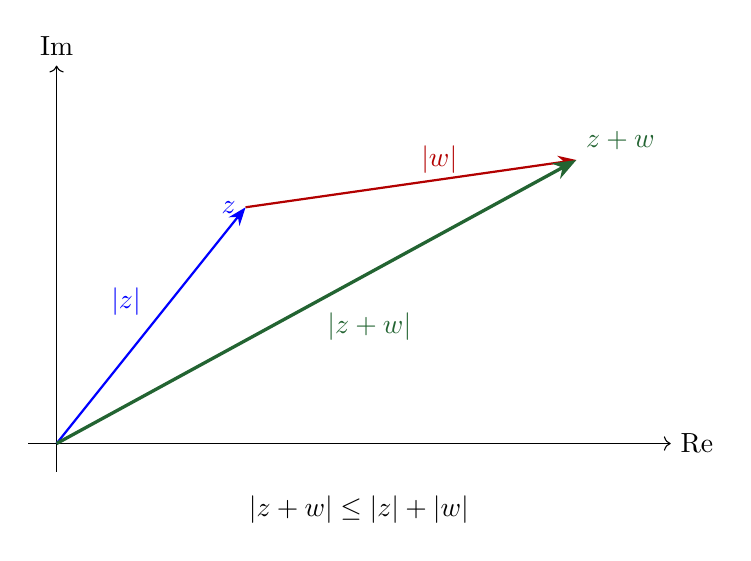
\begin{tikzpicture}[scale=1.2]
    % Axes
    \draw[->] (-0.3,0) -- (6.5,0) node[right]{Re};
    \draw[->] (0,-0.3) -- (0,4) node[above]{Im};
    % Points
    \coordinate (O) at (0,0);
    \coordinate (Z) at (2,2.5);
    \coordinate (W) at (3.5,0.5);
    \coordinate (ZW) at (5.5,3);
    % Vectors
    \draw[-{Stealth}, thick, blue] (O) -- (Z) node[midway, above left]{$|z|$};
    \draw[-{Stealth}, thick, red!70!black] (Z) -- (ZW) node[midway, above right]{$|w|$};
    \draw[-{Stealth}, thick, proofcolor, line width=1.2pt] (O) -- (ZW) node[midway, below right]{$|z+w|$};
    % Labels
    \node[blue, left] at (Z) {$z$};
    \node[proofcolor, above right] at (ZW) {$z+w$};
    % Inequality
    \node at (3.2,-0.7) {$|z+w| \leq |z| + |w|$};
  \end{tikzpicture}
  \end{center}

  \note{
    Here is the geometric meaning. We have the vector "z" shown in blue, and
    the vector "w" shown in red, placed tip to tail. The green vector from the
    origin to "z" plus "w" is the sum. The triangle inequality says that the
    length of the green side, the direct path, cannot exceed the total length
    of the blue and red sides, the indirect path through "z". This is exactly
    the statement that one side of a triangle is at most the sum of the
    other two sides. We now move on to the final topic of this section:
    the Schwarz inequality.
  }
\end{frame}

% =============================================================================
% NOTATION 1.34
% =============================================================================

\section{Summation Notation and the Schwarz Inequality}

\begin{frame}{Notation 1.34: Summation}
  \begin{defblock}{Notation 1.34}
    If $x_1, \dots, x_n$ are complex numbers, we write
    \[
      x_1 + x_2 + \cdots + x_n = \sum_{j=1}^{n} x_j.
    \]
  \end{defblock}

  \note{
    Before we state the Schwarz inequality, we introduce the standard
    summation notation. The capital sigma denotes a sum over the index j
    running from 1 to n. This is purely a notational convenience, but it
    will make the upcoming theorem statement much more compact. Now
    let's state the Schwarz inequality.
  }
\end{frame}

% =============================================================================
% THEOREM 1.35: SCHWARZ INEQUALITY
% =============================================================================

\begin{frame}{Theorem 1.35: The Schwarz Inequality}
  \begin{thmblock}{Theorem 1.35 (Schwarz Inequality)}
    If $a_1, \dots, a_n$ and $b_1, \dots, b_n$ are complex numbers, then
    \[
      \left|\sum_{j=1}^{n} a_j \bar{b}_j\right|^2 \leq \sum_{j=1}^{n} |a_j|^2 \;\sum_{j=1}^{n} |b_j|^2.
    \]
  \end{thmblock}

  \note{
    This is the Schwarz inequality, one of the most important inequalities
    in all of mathematics. It says that the absolute value squared of the
    inner product of two sequences of complex numbers is at most the product
    of their squared norms. Let's see the proof.
  }
\end{frame}

% --- Proof of Schwarz: Setup ---
\begin{frame}{Proof of Theorem 1.35 --- Setup}
  \begin{proofblock}{Setup}
    Write:
    \[
      A = \sum |a_j|^2, \qquad B = \sum |b_j|^2, \qquad C = \sum a_j \bar{b}_j.
    \]

    \vspace{0.3em}
    \textbf{Trivial case:} If $B = 0$, then $b_1 = \cdots = b_n = 0$ and the inequality holds.

    \vspace{0.3em}
    \textbf{Assume} $B > 0$.
  \end{proofblock}

  \note{
    We introduce shorthand: "A" for the sum of absolute values of "a" "j" squared,
    "B" for the sum of absolute values of "b" "j" squared, and "C" for the sum
    "a" "j" times "b" "j" bar. If "B" is zero, then all the "b" "j"'s are zero, both sides
    of the inequality are zero, and there is nothing to prove. So we assume
    "B" is positive. Now here comes the key trick.
  }
\end{frame}

% --- Proof of Schwarz: Key computation ---
\begin{frame}{Proof of Theorem 1.35 --- Key Computation}
  \begin{proofblock}{The trick}
    Expand $\displaystyle\sum |Ba_j - Cb_j|^2$:
    \begin{align*}
      \sum |Ba_j - Cb_j|^2 &= B^2 \sum |a_j|^2 - B\bar{C}\sum a_j\bar{b}_j - BC\sum \bar{a}_j b_j + |C|^2 \sum |b_j|^2 \\
                            &= B^2 A - B|C|^2 \\
                            &= B(AB - |C|^2)
    \end{align*}
  \end{proofblock}

  \note{
    Here is the heart of the proof. Consider the sum of the absolute values
    of "B" "a" "j" minus "C" "b" "j", all squared. Each term in this sum is nonnegative,
    since it is a squared absolute value. We expand using the properties of
    conjugation and the definitions of "A", "B", and "C". After simplification,
    the expression reduces to "B" times the quantity "A" "B" minus the absolute
    value of "C" squared. Now we can finish the argument.
  }
\end{frame}

% --- Proof of Schwarz: Conclusion ---
\begin{frame}{Proof of Theorem 1.35 --- Conclusion}
  \begin{proofblock}{Conclusion}
    Each $|Ba_j - Cb_j|^2 \geq 0$, so
    \[
      B(AB - |C|^2) \geq 0.
    \]
    Since $B > 0$, divide both sides by $B$:
    \[
      \boxed{AB - |C|^2 \geq 0 \qquad\Longleftrightarrow\qquad |C|^2 \leq AB}
    \]
  \end{proofblock}

  \note{
    Since every term in the sum is nonnegative, the entire sum is nonnegative,
    so "B" times "A" "B" minus the absolute value of "C" squared is nonnegative. We
    assumed "B" is positive, so we can divide by "B" and conclude that "A" "B" minus
    the absolute value of "C" squared is nonnegative. Rearranging, the
    absolute value of "C" squared is at most "A" times "B", which is exactly the
    Schwarz inequality. Notice the elegance of the proof: the key idea was
    to introduce the quantity "B" "a" "j" minus "C" "b" "j", which is designed to
    telescope nicely. Let's now summarize the key ideas from this section.
  }
\end{frame}

% =============================================================================
% SUMMARY
% =============================================================================

\section{Summary}

% --- Build 1/4 ---
\begin{frame}{Summary}
  \textbf{Key takeaways from this section:}
  \begin{itemize}
    \item Complex numbers are ordered pairs $(a,b)$ of reals, forming a \alert{field} $\mathbb{C}$
  \end{itemize}

  \note{
    Let's review what we covered in this section. First, we defined complex
    numbers as ordered pairs of real numbers, gave them addition and
    multiplication rules, and proved that the resulting system is a field.
    The key ingredients were the additive identity zero, zero, the
    multiplicative identity one, zero, and the formula for the multiplicative
    inverse involving "a" squared plus "b" squared.
  }
\end{frame}

% --- Build 2/4 ---
\begin{frame}{Summary}
  \textbf{Key takeaways from this section:}
  \begin{itemize}
    \item Complex numbers are ordered pairs $(a,b)$ of reals, forming a \alert{field} $\mathbb{C}$
    \item $\mathbb{R} \subset \mathbb{C}$ via $(a,0) \leftrightarrow a$; \; $i = (0,1)$ with $i^2 = -1$
  \end{itemize}

  \note{
    Second, we showed that the reals embed naturally into the complex numbers
    as pairs with zero second component. The imaginary unit "i" equals the pair
    zero, one, and its square is negative one. This gives us the familiar
    "a" plus "b" "i" notation, which is completely equivalent to the ordered pair
    notation. We also developed important tools for working with these
    numbers.
  }
\end{frame}

% --- Build 3/4 ---
\begin{frame}{Summary}
  \textbf{Key takeaways from this section:}
  \begin{itemize}
    \item Complex numbers are ordered pairs $(a,b)$ of reals, forming a \alert{field} $\mathbb{C}$
    \item $\mathbb{R} \subset \mathbb{C}$ via $(a,0) \leftrightarrow a$; \; $i = (0,1)$ with $i^2 = -1$
    \item Conjugation ($\bar{z} = a - bi$) and absolute value ($|z| = \sqrt{a^2+b^2}$) satisfy the \alert{triangle inequality}
  \end{itemize}

  \note{
    Third, we introduced conjugation and the absolute value, and proved
    the triangle inequality: the absolute value of a sum is at most the
    sum of the absolute values. The absolute value measures distance from
    the origin in the complex plane, and the triangle inequality captures
    a fundamental geometric fact about distances. And there was one more
    major result.
  }
\end{frame}

% --- Build 4/4 ---
\begin{frame}{Summary}
  \textbf{Key takeaways from this section:}
  \begin{itemize}
    \item Complex numbers are ordered pairs $(a,b)$ of reals, forming a \alert{field} $\mathbb{C}$
    \item $\mathbb{R} \subset \mathbb{C}$ via $(a,0) \leftrightarrow a$; \; $i = (0,1)$ with $i^2 = -1$
    \item Conjugation ($\bar{z} = a - bi$) and absolute value ($|z| = \sqrt{a^2+b^2}$) satisfy the \alert{triangle inequality}
    \item The \alert{Schwarz inequality}: $\left|\sum a_j \bar{b}_j\right|^2 \leq \sum |a_j|^2 \sum |b_j|^2$
  \end{itemize}

  \vspace{1em}
  \textbf{Coming up next:} Euclidean Spaces --- generalizing $\mathbb{C}$ to $\mathbb{R}^k$.

  \note{
    Finally, we proved the Schwarz inequality, which bounds the inner
    product of two sequences by the product of their norms. This inequality
    will be essential when we study Euclidean spaces in the next section,
    where we generalize from the complex plane to higher-dimensional real
    vector spaces. Thank you for watching.
  }
\end{frame}

\end{document}
